\subsection{Evaluation der ähnlichen Hotels}
\label{subsec:Evaluation_1}
Der vorliegende Datensatz ist nun verfügbar, und grundsätzlich kann die Modellierung fortgesetzt werden. Allerdings stellt sich die Frage, ob die identifizierten Hotels tatsächlich ähnlich zum ursprünglichen Hotel sind. Es ist von entscheidender Bedeutung, nachzuweisen, dass die ausgewählten Hotels auf irgendeine Weise miteinander vergleichbar sind. Aus diesem Grund wird im nachfolgenden Abschnitt ein Mechanismus entwickelt, um die Ähnlichkeit der Hotels zu überprüfen und zu gewährleisten.
\newline
\newline
Angesichts des angestrebten Ziels, nämlich der dynamischen Generierung von Preisen, wurde zunächst in Erwägung gezogen, die Preise der einzelnen Hotels zu vergleichen. Zu diesem Zweck wurde initial ein \emph{Dataframe} erstellt, das sämtliche gültigen Hotels sowie ihre Preisinformationen für einen bestimmten Zeitraum umfasst.
\newpage
\begin{figure}[h]
    \centering
    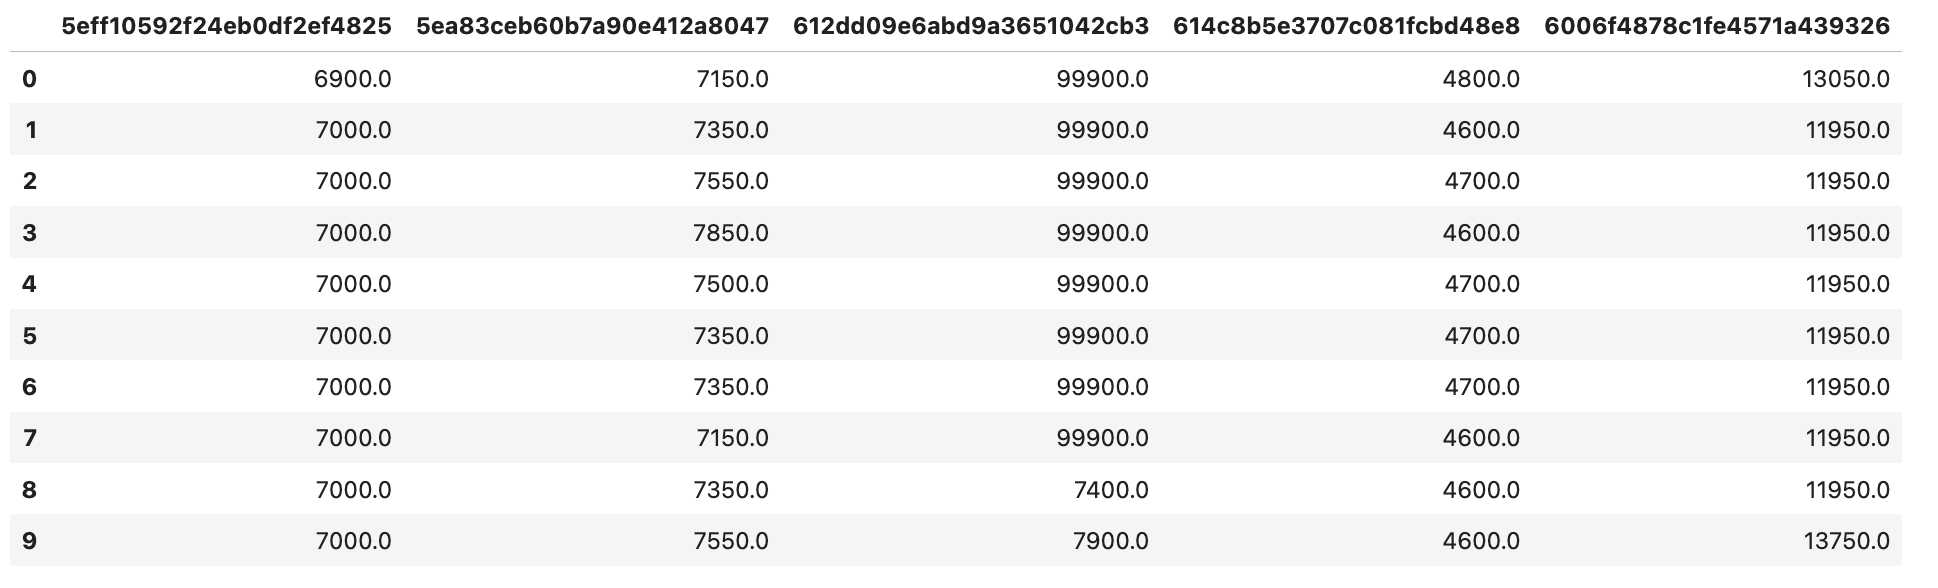
\includegraphics[width=0.9\textwidth, center]{all_prices.png}
    \caption[Preise von allen Hotels für das Jahr 2022]{Preise von allen Hotels für das Jahr 2022}
    \label{img:all_prices}
\end{figure}

Abbildung \ref{img:all_prices} zeigt einen exemplarischen Auszug aus dem DataFrame. Zudem wurde anhand diesem DataFrame noch die dazugehörige Korrelationsmatrix erstellt. Die Korrelationsmatrix ist dafür da, um Zusammenhänge zwischen den Vektoren zu finden. Dabei beschreibt ein Wert nahe 1 einen hohen positiven Zusammenhang der zwei Vektoren und ein Wert nahe -1 einen hohen negativen Zusammenhang der zwei Vektoren. Ein Korrelationswert gegen 0 beschreibt keinerlei Zusammenhang der Vektoren \cite{Team.03.05.2020}. Die Vermutung legt nah, dass wenn die Preise von 2 Hotels korrelieren und die Preise sich überschneiden, so müssten das ähnliche Hotels sein.
\newline
\newline
Diese Vermutung soll dementsprechend mit einigen Hotels getestet werden:
\begin{figure}[h]
    \centering
    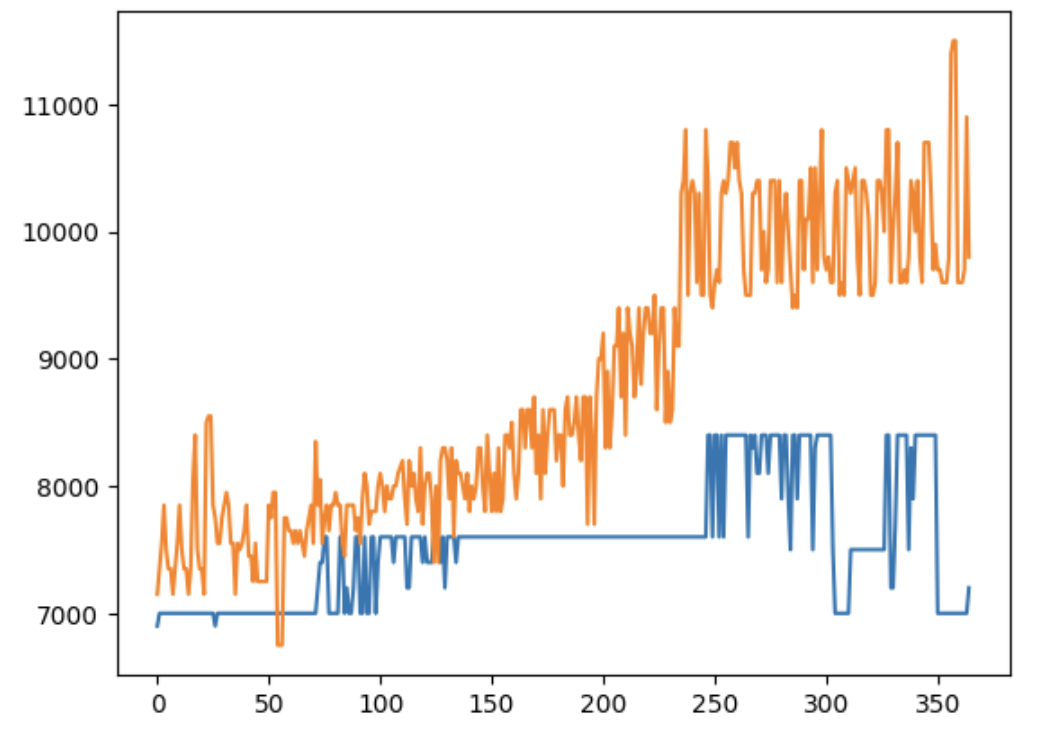
\includegraphics[width=0.9\textwidth, center]{preise_zwei_hotels.png}
    \caption[Visualisierung der Preise zweier Hotels]{Visualisierung der Preise zweier Hotels}
    \label{img:preise_zwei_hotels}
\end{figure}

\begin{figure}[h]
    \centering
    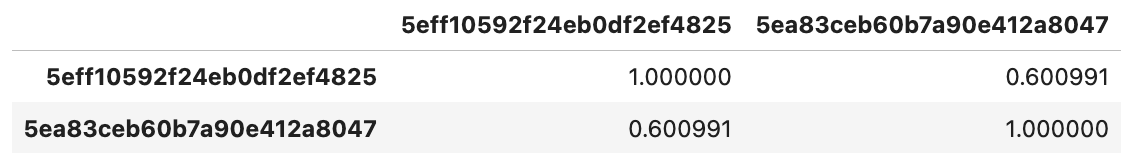
\includegraphics[width=1\textwidth, center]{corr_values_ex.png}
    \caption[Korrelationswerte der zwei Hotels]{Korrelationswerte der zwei Hotels}
    \label{img:corr_values_ex}
\end{figure}

Abbildung \ref{img:preise_zwei_hotels} illustriert den Preisverlauf von zwei Hotels im Jahr 2022, während Abbildung \ref{img:corr_values_ex} die Korrelation zwischen diesen beiden Hotels zeigt. Der festgestellte Korrelationswert von 0,6 erweist sich als bemerkenswert, insbesondere vor dem Hintergrund, dass die Preise in Abbildung \ref{img:preise_zwei_hotels} beträchtlich voneinander abweichen. Infolgedessen wurde die Überlegung angestellt, die Preise zu skalieren und daraufhin miteinander zu vergleichen. Entscheidend für ähnliche Hotels ist lediglich die Tendenz, wie sich die Preise verhalten. 
\newline
\newline
Werden die Preise nun skaliert ändert sich an der Korrelation nichts und die skalierten Preise sehen nun wie folgt aus:

\begin{figure}[h]
    \centering
    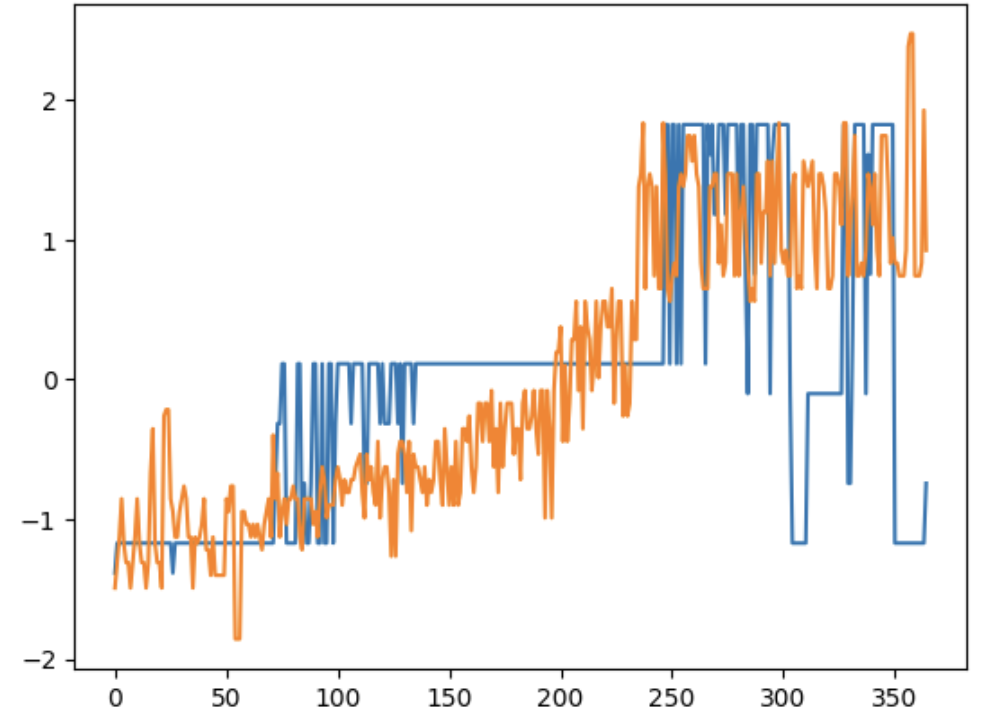
\includegraphics[width=1\textwidth, center]{scaled_preise_zwei_hotels.png}
    \caption[Visualisierung der Skalierten Preise zweier Hotels]{Visualisierung der Skalierten Preise zweier Hotels}
    \label{img:scaled_preise_zwei_hotels}
\end{figure}

Eine zusätzliche Betrachtung ergab die Frage, ob ein ähnliches Muster nicht auch durch die Verwendung des RevPAR erzielt werden könnte. Die Verwendung des RevPAR-Werts erscheint in diesem Kontext sinnvoller als die ausschließliche Berücksichtigung der Zimmerpreise, da das nachfolgende Modell letztendlich darauf abzielt, den RevPAR-Wert vorherzusagen.
\newline
\newline
Im Folgenden werden die gleichen zwei Hotels mit dem RevPAR-Wert verglichen:

\begin{figure}[h]
    \centering
    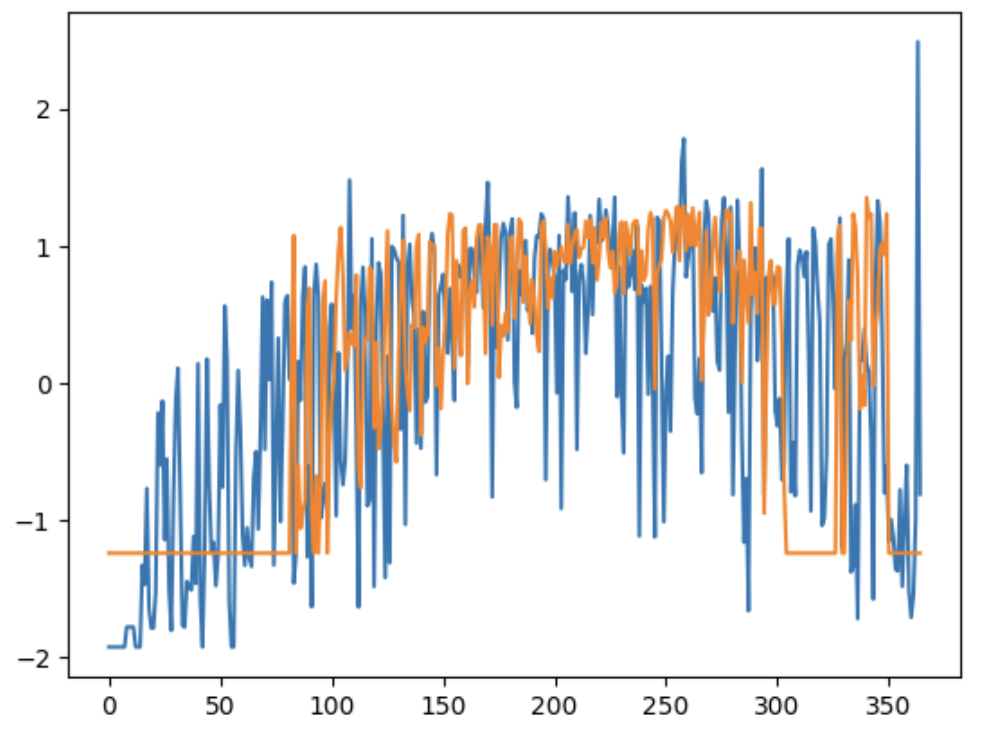
\includegraphics[width=1\textwidth, center]{scaled_revpar_zwei_hotels.png}
    \caption[Visualisierung der Skalierten RevPAR-Werte zweier Hotels]{Visualisierung der Skalierten RevPAR-Werte zweier Hotels}
    \label{img:scaled_revpar_zwei_hotels}
\end{figure}

\begin{figure}[h]
    \centering
    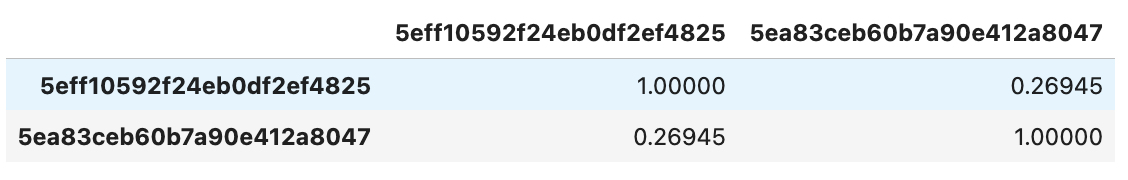
\includegraphics[width=1\textwidth, center]{corr_revpar_values_ex.png}
    \caption[Korrelationswerte der RevPAR-Werte zweier Hotels]{Korrelationswerte der RevPAR-Werte zweier Hotels}
    \label{img:corr_revpar_values_ex}
\end{figure}

Abbildung \ref{img:corr_revpar_values_ex} offenbarte einen abweichenden Korrelationswert im Vergleich zu demjenigen, der bei der Betrachtung der Preisentwicklung ermittelt wurde. Daraufhin wurde die Entscheidung getroffen, dass der Korrelationswert der RevPAR-Werte als aussagekräftiger betrachtet wird als derjenige der reinen Preisentwicklung. Infolgedessen wurde festgelegt, dass dieser Wert als Evaluation für die Ähnlichkeit zwischen den Hotels herangezogen wird.
\newline
\newline
Dieser Korrelationswert der RevPAR-Werte kann lediglich zur Evaluation der Modelle verwendet werden, da dieser Korrelationswert für ein Hotel nicht vorhanden ist. 